% This is "sig-alternate.tex" V1.9 April 2009
% This file should be compiled with V2.4 of "sig-alternate.cls" April 2009
%
% This example file demonstrates the use of the 'sig-alternate.cls'
% V2.4 LaTeX2e document class file. It is for those submitting
% articles to ACM Conference Proceedings WHO DO NOT WISH TO
% STRICTLY ADHERE TO THE SIGS (PUBS-BOARD-ENDORSED) STYLE.
% The 'sig-alternate.cls' file will produce a similar-looking,
% albeit, 'tighter' paper resulting in, invariably, fewer pages.
%
% ----------------------------------------------------------------------------------------------------------------
% This .tex file (and associated .cls V2.4) produces:
%       1) The Permission Statement
%       2) The Conference (location) Info information
%       3) The Copyright Line with ACM data
%       4) NO page numbers
%
% as against the acm_proc_article-sp.cls file which
% DOES NOT produce 1) thru' 3) above.
%
% Using 'sig-alternate.cls' you have control, however, from within
% the source .tex file, over both the CopyrightYear
% (defaulted to 200X) and the ACM Copyright Data
% (defaulted to X-XXXXX-XX-X/XX/XX).
% e.g.
% \CopyrightYear{2007} will cause 2007 to appear in the copyright line.
% \crdata{0-12345-67-8/90/12} will cause 0-12345-67-8/90/12 to appear in the copyright line.
%
% ---------------------------------------------------------------------------------------------------------------
% This .tex source is an example which *does* use
% the .bib file (from which the .bbl file % is produced).
% REMEMBER HOWEVER: After having produced the .bbl file,
% and prior to final submission, you *NEED* to 'insert'
% your .bbl file into your source .tex file so as to provide
% ONE 'self-contained' source file.
%
% ================= IF YOU HAVE QUESTIONS =======================
% Questions regarding the SIGS styles, SIGS policies and
% procedures, Conferences etc. should be sent to
% Adrienne Griscti (griscti@acm.org)
%
% Technical questions _only_ to
% Gerald Murray (murray@hq.acm.org)
% ===============================================================
%
% For tracking purposes - this is V1.9 - April 2009

\documentclass{sig-alternate}
  \pdfpagewidth=8.5truein
  \pdfpageheight=11truein
  
\setcounter{secnumdepth}{4}

\begin{document}
\title{Feature Based Opinion Mining: A Modern Approach}

\numberofauthors{3}
\author{
\alignauthor
Eke, Norbert\\
       \email{norbert.eke@alumni.ubc.ca}
	\email{UBC Okanagan}
% 2nd. author
\alignauthor Andrews, Jeffrey\\
       \email{jeff.andrews@ubc.ca}
	\email{UBC Okanagan}
% 3rd. author
\alignauthor Mohamed, Abdallah\\
       \email{abdallah.mohamed@ubc.ca}
	\email{UBC Okanagan}
}

%\date{\today}
% Just remember to make sure that the TOTAL number of authors
% is the number that will appear on the first page PLUS the
% number that will appear in the \additionalauthors section.


\maketitle
\begin{abstract}
In a world where customers can buy products with a few clicks online, future customers must consider the opinions and satisfaction levels of previous customers. In order to allow one to understand what previous customers have said, the design of an automated technique that summarizes opinions of thousands of customers is desirable. A promising technique has been developed that combines continuous vector representation models, natural language processing techniques and statistical machine learning models. This technique has been tested on labelled datasets and it extracts over 80\% of opinions correctly. Future research can focus on improving the technique's limitations on edge cases.
\end{abstract}

\terms{Opinion Mining, Feature Extraction, Opinion Detection}
\keywords{Word Vector Spaces, Statistical Machine learning, Natural Language Understanding, Word Embeddings}

\section{Introduction}
Customer reviews are essential for establishing what previous customers' opinions and satisfaction levels are towards a product, entity, event or experience related to a brand or company. Nowadays, one can find hundreds of online reviews for most commercial products that are sold online. Difficulties arise when a person is trying to analyze and interpret a large number of customer reviews. Categorizing and summarizing customer opinions based on features found in a reviews is the problem commonly known as feature-based opinion mining of customer reviews. 
Feature-based (customer) opinion mining consists of three main components: feature, opinion and opinion mining. A feature is the characteristics or aspects of a product. An opinion is a subjective belief, which is the result of emotion or interpretation of facts and opinion mining is the detection of patterns among opinions. Feature based opinion mining is a special kind of text summarization, in which one is trying to identify specific features of the product that customers have positive or negative opinions on. Essentially, a feature-based opinion mining system provides a summary of all the positive and negative opinions found about each feature of the product present in customer reviews.
This research addresses a number of concerns related to customer reviews. There are too many reviews about products on the internet. In fact there are over 26 thousand reviews posted on Yelp every minute (Shrestha, 2016). An assumption can be made that no one reads all of the reviews, and it can be  backed up with some statistics: 88\% of consumers form an opinion by reading up to 10 reviews (Shrestha, 2016). One can made the argument that people who only read a few reviews will not get a fully accurate representation of what everyone's opinion is about a certain product. The research problem consists of needing a way to interpret the content of millions of reviews, without reading them all. The main goal of this research project is to come up with a technique that automatically detects opinion phrases straight from the customer reviews. Such a technique provides a summary of all opinions, which serves as convenience for customers, business intelligence for companies and enhances business customer relationships.

\section{Previous Work}

\subsection{Overview of previous work}
Hu \& Liu (2004) were the first researchers to formulate the problem of opinion detection as a natural language processing problem. They named this type of problem 'feature based opinion summarization'. Hu and Liu's approach consisted of a system of algorithms that make use of several data mining and natural language processing techniques in order to extract specific features from customer reviews. Their objective was to produce a feature-based summary of a large number of customer reviews. In their paper, Hu and Liu also mentioned that they aim to find what people like and dislike about a given product. This first approach by Hu and Liu was considered the golden standard in mid 2000s, and almost all recent approaches share some common characteristic with the original work. 

In 2006, Ku et al. proposed an algorithm for opinion extraction, summarization, and tracking. The work of Hu and Liu was the basis for an approach presented by Ren and Wang, who suggested that reviews could be pre-processed automatically and customers could be provided with the generalized information (Ren \& Wang, 2007). Later on, Pang \& Lee (2008) wrote about experimenting with natural language understanding models, various classification techniques and multi-document opinion-oriented summarization techniques. 

In the first five to ten years after Hu and Liu (2004)'s work, almost every researcher approached the problem using natural language processing and understanding, sentiment classification and summarization techniques. Few researchers have looked at feature based opinion mining, as a problem which could be solved using artificial intelligence, particularly, machine learning.

In 2013, Mikolov et al. proposed two models for computing continuous vector representations of words. These models are machine learning models, which are trained to reconstruct linguistic contexts of words by converting words into multidimensional word vectors. Mikolov et al. (2013)'s model encodes the meaning of words, and relationship between words in such a way that contextual meaning of the text is preserved in the form of high dimensional vectors.

The above mentioned natural language processing approaches and many others contributed enormously towards solving the problem of feature-based opinion summarization of customer reviews. However, one might say that linguistic machine learning models could potentially offer a better solution towards more accurate feature based opinion mining. Vector representation of words models were not applied to this problem, and the use of such models could potentially decipher the positive and negative opinions or experiences customers have had.

\subsection{In-depth analysis of previous approaches}
In terms of previous feature-based opinion mining systems there are a variety of approaches taken by numerous researchers. Hu and Liu's approach in 2004 started out the trend of natural language processing algorithms towards detection of opinion phrases. Their approach consisted of Parts of Speech (POS) tagging, then using a version of the Apriori algorithm (Agrawal \& Srikant, 1994) to obtain the frequently occurring nouns. Most frequent nouns would become candidate features, or aspects. All the candidate features need to go through two phases of candidate feature pruning. The first phase is called 'compactness pruning', and it checks candidate aspects that are more than two words and removes the non-compact, longer phrases. The second phase of the pruning process is called 'redundancy pruning' and it removes aspects/features with a p-support less than 3, where p-support is "number of sentences that a feature appears in as a noun or noun phrase" (Hu \& Liu, 2004, pp 171). After all candidate features have been pruned, an opinion phrase is formed by looking up the nearest adjective of the feature. Last step in Hu and Liu's approach is to look up the polarity of the descriptor word (modifier) from a sentiment lexicon. 

Popescu \& Etzioni (2007) came up with a slightly different approach in 2007. Their approach was called Opine and they incorporated a 'Point-wise Mutual Information' (PMI) scoring system inside Hu and Liu's algorithm system, which resulted in a 22\% improvement on opinion phrase detection. Popescu and Etzioni's Opine system "evaluates each noun phrase by computing the PMI scores between the phrase and meronymy discriminators associated with the product class." (Popescu \& Etzioni, 2007, pp 341). The PMI score between phrases are calculated from web search engine result counts (Turney, 2001). 

Scaffidi et al. (2007) built on this work by calculating the probability of an identified frequent noun to be a feature, which improved Popescu and Etzioni's version of a feature based opinion mining system. They called their approach the 'Red Opal'. 

In 2009, a handful of researchers introduced some machine learning techniques into the problem of feature based opinion mining. Go et al. (2009) incorporated machine learning classifiers such as Naive Bayes, Maximum Entropy classifiers and Support Vector Machines to classify features, opinion phrases and their polarity. Go et al.'s work was one of the first steps made towards the transition of using more machine learning techniques instead of natural language processing techniques to solve the problem of feature based opinion mining.

In 2010, Moghaddam and Ester introduced the Opinion Digger, a feature based opinion mining system that uses data mining to identify potential aspects/features. This was one of the systems that changed the approach, by mainly using data mining tools, instead of natural language processing techniques. The Opinion Digger finds frequent nouns, then mines opinion patterns. After some patterns have been identified, it filters out non-aspect/non-feature words, then rates aspects/features using a customized version of the k-nearest neighbour (kNN) algorithm. Once all the potential features/aspects have been found, Moghaddam and Ester suggest that "sentiments are usually the nearest adjectives in the same sentence segment, which describe the quality of the aspect" (Moghaddam \& Ester, 2010). In this case, quality of aspects is referred to opinion modifiers or descriptor words.

Zhao et al. (2011) approached the problem from a different perspective. Using Latent Dirichlet allocation techniques applied to some Twitter data, they were able to come up with an algorithm to extract key phrases, that could potentially be opinion phrases. Their algorithm consisted of candidate key phrase generation based on keyword ranking, then finish it off by extracting key phrases by using a 'Topical PageRank' (TPR) scoring system to rank key phrases. This approach changed the academic perspective on key phrase extraction.

Spina et al. (2012) formulated the problem as an information retrieval and opinion target identification, and they applied four different methods to solve the problem. They looked at Term Frequency - Inverse Document Frequency (TF-IDF) ratios and log-likelihood ratios to identify patterns from words in the data, then used 'parsimonious language models' (PLM) and opinion oriented methods that extract targets of opinions to generate topic specific sentiment lexicons. Spina et al.'s work should be applied to any feature based opinion mining system, since it solves the issue of what/who is the opinion target. Spina et al. reported that the TF-IDF ratios worked better that the other three methods.

Das and Kannan took a more statistical approach to the problem by looking at "topical aspects in microblogs" (Das \& Kannan, 2014). Their approach involved looking at local and global indicators within the data. Global topical aspect indicators looked at uniqueness of words by measuring how strongly a phrase is correlated with a target entity. Local topical aspect indicators used Gaussian mixture models and some probabilistic models combined with the Expectation-maximization (EM) algorithm to identify observations like burstiness and diversity of phrases. In this case, burstiness is meant to measure how frequently a phrase is used, while diversity is meant to measure how differently a phrase is used.

In 2016, Ejieh proposed an algorithm called Microblog Aspect Miner (MAM), which incorporates data science techniques into a feature based opinion mining system. The MAM algorithm uses Mikolov et al.'s (2013) word2vec model to convert words into high dimensional vectors. These vectors will serve as features for a K-means clustering algorithm, in order to isolate a cluster of frequent nouns. Ejieh calculates "Aspect-Product Similarity Threshold' values, which are used to 'rank how relevant an aspect/feature is to a product" (Ejieh, 2016). Ejieh also introduced a 'subjectivity module' to detect if a post expresses an opinion, and he noted that non-opinion words will be discarded. All of these components improved the overall performance of opinion detection system, while it inspired some of the components of technique designed in this research project and described in section 4. 

Finally, in 2017 Sanger et al. have looked at expanding a document's dictionary by adding in the synonyms of words used in the text. They called this technique "synonym expansion" (Sanger et al., 2017). They have also performed clustering of words, after the synonyms have been added to the document's dictionary. Their results are promising and their system of algorithms could be considered to be added inside a feature extraction natural language processing technique.

\section{Research Question and Objectives}
The main goal of this research project was designing a novel approach that could analyze customer reviews and gain valuable insight into customer review. Such an approach would be looking into what exactly customers are saying about a specific product, event or experience related to a brand or company. This research will focus on combining a vector representations of words model with statistical classification models and natural language processing techniques  to produce a unique system of algorithms solving the feature based opinion mining problem. This modern approach applied to the problem of feature-based opinion summarization could potentially extract valuable information from customer reviews.
In order to design a technique that accomplished the above goals, the approach needs to be developed and validated on one or more annotated benchmark data sets. After understanding the performance, the technique could be used to analyze new data sets of real customer reviews in which customers express their positive and negative experiences. This research project initially focused on answering the following questions: 

Q1: 'What are the benefits of continuous vector representation of word models for feature-based opinion summarization of customer reviews?'

Q2: 'Can enough valuable insight be extracted from customer reviews? Can this insight be grouped or categorized into different kinds of opinions that have been said about a product/entity/event/experience related to a company ?'

Q3: 'What kind of limitations would such a "customer opinion categorizer and summarizer" have?'

\section{Technique designed}
Before getting too far ahead, one needs to get familiar with opinion phrases, in order to understand the technique. Opinion phrases consists of feature word(s), like 'touch screen' and a descriptor word, like 'good'. Figure 1 illustrates the concept of opinion phrases. \\
\begin{figure}
\centering
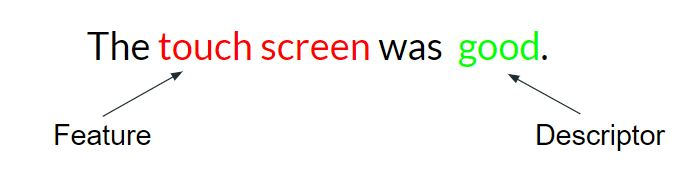
\includegraphics[scale=0.65]{images/FD_words.JPG}
\caption{Opinion phrases are feature - descriptor word pairs, like 'good - touch screen'.}
\end{figure}

\subsection{Textual Data}
In this project two subsets of annotated datasets have been used for developing and testing the technique: Computer reviews dataset (Hu \& Liu, 2004) and TripAdvisor Hotel reviews dataset (Wang et al., 2010; 2011). Another dataset named the "Adjective-Noun Word pair benchmark dataset" (Borth et al., 2013) has played an important role in this project, by serving as training data for machine learning classification models.

\subsection{Text Preprocessing}
There is no silver bullet algorithm for text preprocessing. There are many kinds of text processing techniques and algorithms used in natural language processing, and all of them are useful for different data cleaning and data processing scenarios. In this research project numerous text processing techniques were used, forming a couple of similar text cleaning algorithm systems. 
In the proposed technique text cleaning was needed for four different purposes: feature extraction (section 4.3.1), processing of words for vector representation of words model (section 4.3.2), dependency parsing (section 4.3.3) and processing of the labelled benchmark datasets (section 4.4.2). Out of these four techniques feature extraction and dependency parsing needed identical text cleaning, while the input for vector representation and processing of benchmark datasets needed a different kind of processing. Essentially, the first kind of processing is more forgiving on cleaning text, thus being called 'soft-processing' in this project, while the second kind of text processing is tougher on cleaning up text, being called 'hard-processing'. The similarities and differences can be seen in the following table.

\begin{figure}
\centering
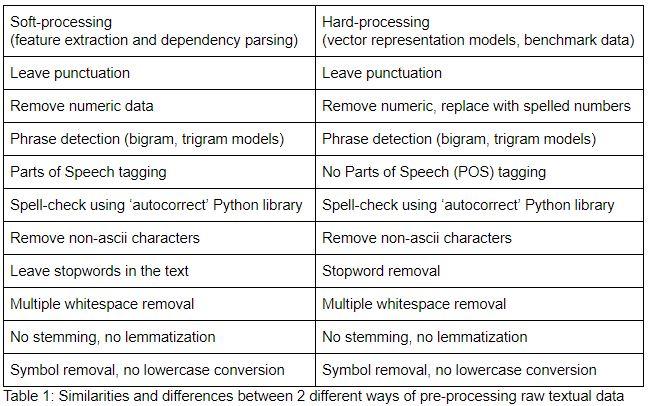
\includegraphics[scale=0.65]{images/text_processing_table.JPG}
\end{figure}

The main difference between the two different ways of preprocessing is the punctuation removal, parts of speech tagging and stopword removal. These differences can be justified by the needs of the technique. Feature extraction and dependency parsing make use of stop-words, punctuation and parts of speech tagging, while word vector representation models and the labelled benchmark datasets do not need the three techniques above mentioned.

\subsection{Interaction between Deep Learning and Natural Language Processing}
\subsubsection{Feature Extraction}
Feature extraction applied in natural language processing has been wildly researched since the early 2000's, and many methods have been developed throughout the years. A small summary of previous works in this area can be found in section 2. Shortly, there are mainly 5 kinds of feature extraction methods: frequency based methods, relation based methods, hybrid methods, supervised learning based methods and topic modelling based methods. Each type of methods have pros and cons. On a personal note, hybrid approaches tend to work the best, by combining multiple approaches together and widening the scope of the algorithm. Any approach that has been tested and it performs well on benchmark datasets is acceptable. For this project's purpose an open source feature extraction package was used, created by Akshay Bansal. The author of the package described his implementation as an "application in the field of natural language processing in order to find and implement a novel algorithm to solve the problem of measuring real-time comments made by users on products" (Bansal, 2014). The whole implementation is available publicly online and it is a hybrid approach combining a relation and frequency based method. For this research project's purposes this implementation of the feature extraction technique was considered good enough in order to proceed forward with the real focus of this project, which is centered around relation vectors (section 4.4.3). Bansal's implementation makes use of natural language processing techniques like parts of speech tagging, tokenization, lemmatization and many others. 
In the implementation of the proposed technique, feature extraction plays quite an important role, however before even running the feature extraction algorithm, the raw input data needs to be cleaned up. For pre-processing the 'soft processing' system of algorithms is preferred over 'hard processing' since the feature extraction algorithms makes use of punctuation, stopwords and parts of speech tagging, which should not be removed from the raw input documents during the pre-processing steps. Once the raw input documents have been cleaned up, the feature extraction algorithm identifies potential features within the text, based on word frequencies and parts of speech tagging. All features extracted will be essential in one of the technique's upcoming step, which is Feature - Dependency Word Linkage described in section 4.5. A demonstration of what feature extraction does can be seen in Figure 2.

\begin{figure}
\centering
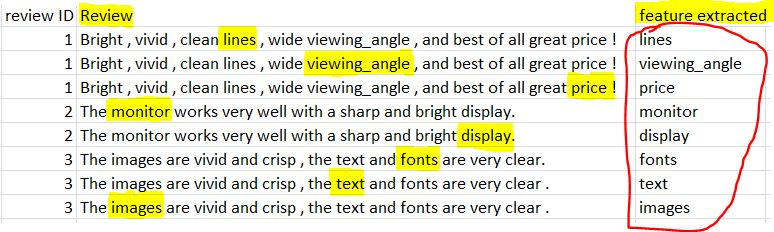
\includegraphics[scale=0.60]{images/feature_extraction.JPG}
\caption{Example of features extracted from sample sentences. The highlighted words represent the features identified in the sample sentence.}
\end{figure}

\subsubsection{Continuous Vector Representations of Words Using Word2Vec}
Word2Vec is Google's deep learning model that allows the computation of vector representations of words. This word2vec model takes a text corpus as input and produces high dimensional word vectors as output. In one of Google's blog posts the algorithm is described as "it constructs a vocabulary from the training text data and then learns vector representation of words. The resulting word vector file can be used as features in many natural language processing and machine learning applications" (Mikolov et al., 2013). 
These word vectors are also called word embeddings, and they are the output of the word2vec model. Essentially, with the help of the word2vec words get turned into high dimensional vectors. The word2vec model is trained to reconstructs the linguistic context of words by placing the vectors of words used in the same context close to each other. Word embeddings are also useful, since they "capture the semantic similarity between words by placing the vectors of similar words closer to each other" (Mikolov et al., 2013). Low dimensionality word embeddings, or word vectors can be visualized in so called word vector spaces. A good example of a simple, three dimensional vector space can be seen in Figure 3.

\begin{figure}
\centering
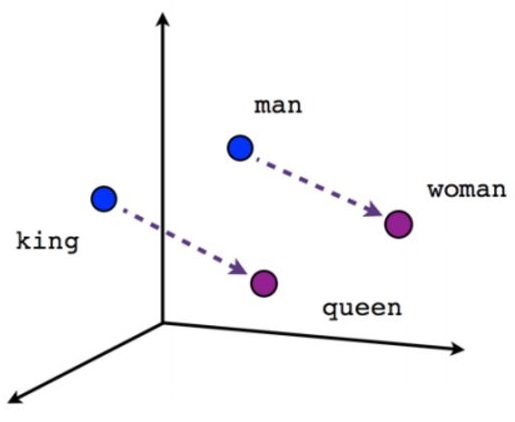
\includegraphics[scale=0.60]{images/vectorSpace.JPG}
\caption{Three dimensional vector space, which contains the vectors 'man', 'woman', 'king', 'queen'. In this three dimensional vector space,  'man' and 'woman' are related to each other the same way as 'king' and 'queen' are related to each other, since the vectors in between them describe the male-female relationship.}
\end{figure}

The word2vec model has 2 different architectures: cbow (continuous bag of words) and skip-gram. The difference between the two architectures is that cbow predicts the current word given the context, while skip-gram predicts the surrounding words given the current word. During the entire length of this research project Google's 300 dimensional pre-trained skip-gram model (Mikolov et al., 2013) was used. This model is a static model that was trained on close to 100 billion words and it contains 300 dimensional vectors for 3 million unique words. 
Throughout the process of this research project this model was used as a static lookup table for the vector representation of a specific word. What this means is that every document to be analyzed was cleaned and pre-processed, then every word from the processed documents was fed into the word2vec deep learning model, allowing the model to output a 300 dimensional vector representation for every unique word in the documents. Sadly, it was close to impossible to properly train a word2vec model just for the purposes of this research project, since these kinds of deep learning models need to learn vector representations of words from text corpuses of billions of words and there was no access to such dataset in this short period of time. Future improvements on the system of algorithms could include the use of an improved word vector representation model or the training of a model that uses a training corpus from the same domain knowledge area as the future textual data to be analyzed.


\subsubsection{Dependency Parsing}
Dependency parsing is a natural language processing technique, which analyzes the textual data syntactically. It looks at the structure of the sentences and builds a dependency tree showing how words relate or depend on other words in the sentence. Dependency parsing can be performed using different methods. Two different methods that have been considered and looked at. The first one makes use of context free grammar (Bird, 2009) and the second methods takes a model based approach. As a personal note, the most accurate dependency parsers come from carefully trained models, like the Stanford Parsing model family (Chen \& Manning, 2014), or modern industry standard models like RedShift (Honnibal, 2013) and Spacy (Honnibal, 2017). For this project's purposes SpaCy python package's dependency parsing model was deemed to be a good fit as it builds dependency trees effectively and efficiently. 
In the technique implemented, before using dependency parsing the 'soft processing' technique mentioned in section 4.2 is used to clean up the documents. For dependency parsing, the 'soft processing' system of algorithms is preferred over 'hard processing' since dependency parsing makes use of punctuation and stopwords, which should not be removed from the raw input documents during the pre-processing steps. SpaCy's dependency parser (Honnibal, 2017) segments the input documents sentence by sentence, labels the parts of speech in the sentences with the help of their internal model, which then builds a dependency tree similar to the one in Figure 4.


\begin{figure}
\centering
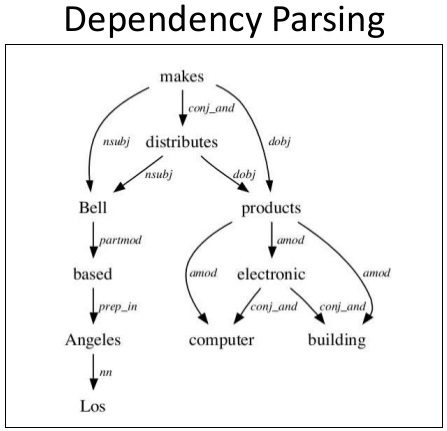
\includegraphics[scale=0.60]{images/dependency-parsing.jpg}
\caption{Sample dependency tree: arrows represent the dependency relation between words.}
\end{figure}
The produced dependency tree is an essential piece of Feature - Dependency Word Linkage described in section 4.5.

\subsection{Supervised Learning}
In order to perform supervised learning, and build 'smart systems of algorithms' that know how to identify opinion phrases, there needed to be an annotated training dataset(s), in which features and descriptors are labelled, so a model could be trained to detect opinion phrases. Such datasets have been identified in section 4.1. 

\subsubsection{Feature Descriptor Relation Vectors}
The main focus of this research project was the relationship between feature words and descriptor words. Keeping textual data as words is not particularly useful. To gain insight into the context of the words used in the customer reviews, words needed to be converted into high dimensional vectors using word embeddings. Using the vector representation of words model, a feature word can be converted into a feature vector and a descriptor word can be converted into a descriptor vector. After converting words into vectors, the relationship between feature and descriptor words can be simplified to the difference between the feature vector and descriptor vector. In this research project, the difference of the two vectors is referred to as the feature descriptor relation vector or just simply, the relation vector. A visualization of how a relation vector can be found in shown below, in Figure 5.

\begin{figure}
\centering
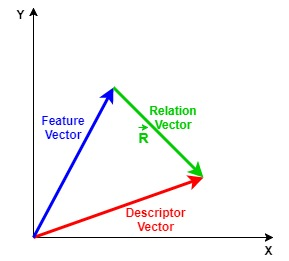
\includegraphics[scale=0.60]{images/relation_vec.jpg}
\caption{Two dimensional visual representation of a feature descriptor relation vector (R vector)}
\end{figure}

These so called relation vectors have some important properties. Not every subtraction of two random vectors has the same features as a relation vector. Through careful analysis of the characteristics and features of these relation vectors it was identified that the difference of all feature and descriptor vectors is in some way different than the difference of two random vectors. The difference of feature and descriptor vectors is an 'encoding' of the semantic relationship between a feature and descriptor word. Two random words' vector  representations' difference does not 'encode' the same semantic relationship as a relation vector does. Thus, there are 2 kinds of relation vectors : real and non-real. A real relation vector is the difference of vectors of valid feature and descriptor vectors. A non-real relation vector is a random word pair encoded in vectors, that makes no sense. For example a real relation vector would be the vector representation of the words 'nice' and 'desk', while a non-real relation vector would be the vector representation of any two words that do not make any semantical sense together, like 'going' and 'desk'. Knowing the difference between a real and a non-real relation vector, one can see how there needs to be a way to differentiate between these 2 types of relation vector, thus the idea of building a relation vector classification model came about (section 4.4.4).

\subsubsection{Training Data Processing}
In the early phases of the research project the use of properly labelled textual data, like the Computer dataset (Hu \& Liu, 2004) or the Hotel dataset (Wang et al., 2010; 2011) was crucial, however the already labelled datasets needed textual data preprocessing. The 'hard processing' technique mentioned in section 4.2 was chosen for the benchmark training data processing. Keeping textual data as words is not useful at all, instead words need to be converted into high dimensional vectors using word embeddings. In order to produce good word embeddings, the removal of punctuation, numbers and stop-words are needed, thus the decision to use 'hard processing' over 'soft processing' was easy to make.


\subsubsection{Feature - Descriptor labelling}
After data preprocessing, labels for feature and descriptor word were needed. These labels usually come from annotated datasets, like Computer dataset (Hu \& Liu, 2004) or the Hotel dataset (Wang et al., 2010; 2011). Some datasets only have the features labelled, some have both features and descriptors labelled. In case descriptors are not labelled, the inconvenient process of a person going through a subset of the labelled data and annotate the descriptor word for the already labelled feature word is needed. In this case one needs to look for the description (what is it said) about the feature word. In order to keep track of feature - descriptor word pairs present in the training documents, one needs to create a table with the columns containing review number, review content, feature word, descriptor word present in a specific review. One needs to recognize that this process is tedious, but it is needed to be done only once, when one is intending on training a Relation Vector Classification Model (section 4.4.4). This whole research project's goal is to design an automated technique that summarizes opinions from thousands of documents. In normal circumstances this process would never be needed, however this project's approach is learning relation vectors through a supervised learning, thus there needs to be some training data.

\subsubsection{Relation Vector Classification Models}
With the use of labelled training data described in section 4.4.2 and 4.4.3 it was possible to train multiple classification models. After some experimentation with training and testing over a dozen kinds of classification models, half a dozen were chosen as the most effective models at classifying real and non-real relation vectors. The models include two LASSO models, one Support Vector Machine (SVM) model, one Bagging model, one Random Forest model, one Linear Discriminant (LDA) model and a Gradient Boosting model. By the end of the research project there were 2 different training datasets, thus there are two models of each kind, one model trained on the first dataset, and the other trained on the second dataset. 
All the models and even the training data will be made public on this research project's GitHub repository (Eke, 2017). The performance of all models listed above is discussed in section 5. Figure 6 shows the logistics behind the supervised relation vector classification models.

\begin{figure}
\centering
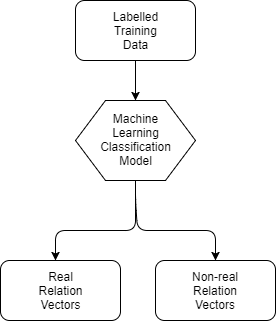
\includegraphics[scale=0.60]{images/machine_learning.png}
\caption{Simple visual representation of the supervised relation vector classification model.}
\end{figure}


\subsection{Feature - Dependency Word Linkage}
The technique's probably most important steps is called the word linkage. Knowing about feature words, descriptor words and relation vectors, one needs to keep in mind that the whole technique is about finding the proper feature descriptor word pairs. This task is getting accomplished by identifying potential relation vectors. The purpose of word linkage is simple: use the output of two previously discussed algorithms, feature extraction and dependency parsing to create candidate relation vectors. The feature extractor identifies all the features in the text, but it does not have a way to find the descriptor word. Word linkage takes care of finding the descriptor words by having the feature extractor work together with the dependency parser. The feature extractor passes all features extracted from the text to the dependency parser, which takes all features and builds a dependency tree for the sentences that each feature is present in. A structural diagram of the word linkage technique is shown, in Figure 7.

\begin{figure}
\centering
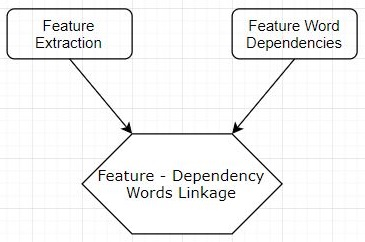
\includegraphics[scale=0.60]{images/linkage.JPG}
\caption{Structural diagram of feature - dependency word linkage.}
\end{figure}

After the feature extractor and dependency parser have finished their job, a dependency tree parser produces a list of words that are dependent to the feature word present in each parsed sentence. The dependency tree parser takes in a dependency tree and returns a list of words that match a custom criteria within the dependency tree. Such a criteria can be defined as return all the word nodes within the tree that are the parent node, grandparent node, sibling nodes and children nodes of the feature word's node. One can call this custom criteria as the 'tree segmentation criteria'. After lots of experimentation the best tree segmentation criteria was found to be the example criteria mentioned above. This process is shown in Figure 8. 

\begin{figure}
\centering
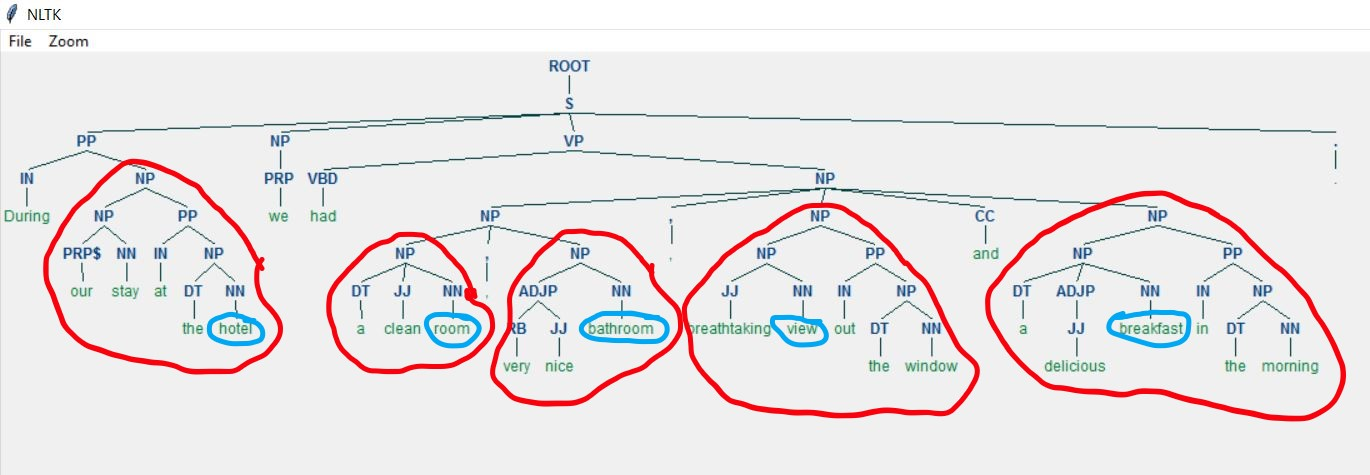
\includegraphics[scale=0.25]{images/dep_tree_parsing.JPG}
\caption{Example of what the dependency tree parser does. The words circled in blue are feature words, and the group of words circled in red are the list of words that the dependency parser picked out to be dependent or related to the feature word.}
\end{figure}

Once the dependency tree parses has done its job, the word linkages can be created by taking each feature vector and 'linking' it with feature word's list of dependency word's vectors. To be more clear, a feature word is paired up with all of the words that depend on the feature word, thus creating many candidate feature - descriptor word pairs, all being encoded in potential relation vectors. There is one flaw: as you can see on the list of words circled in red in Figure 8, not all words dependent on the feature are descriptor words. Some word pairs' vector representations are real relation vectors, but most of them are non-real relation vectors. The next section deals with filtering out the non-real relation vectors.

\subsection{Feature Descriptor Filtering}
In Section 4.4.4 it was described how a few relation vector classification models were created. These models have been trained with the sole purpose of classifying real and non-real relation vectors. The classification process comes along really handy when one needs to filter out all the non-real relation vectors created in the word linkage process. The filtering process is simple: feed into one of the classification models all the candidate relation vectors created by the word linkage algorithm. The machine learning model will throw out all the relation vectors classified as non-real, keeping only the vectors classified as real relation vectors, thus finding all the real feature - descriptor word pairs. A logistics diagram of how this is achieved can be seen in Figure 9. 

\begin{figure}
\centering
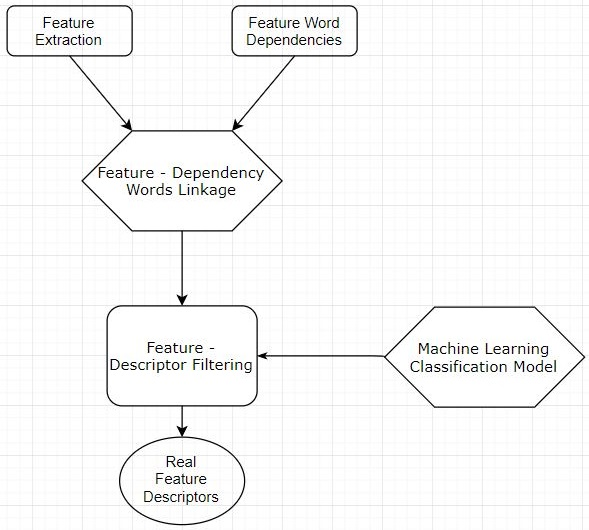
\includegraphics[scale=0.60]{images/opinion_filtering.JPG}
\caption{Logistics of how the non-real feature descriptor relation vectors get filtered out using a machine learning classification model of one's choice.}
\end{figure}

\subsection{Opinion Phrase Polarity}
Once all the real opinion phrases have been identified by the relation vector classification model, the only few steps left are classifying the polarity of opinion phrases, creating a feature breakdown of all opinion phrases, so they form clusters for each individual feature and creating a summary of all the positive and negative opinion phrases, so summarizing everything as a feature based opinion mining system.
Classifying opinion phrase polarity can be considered a sentiment analysis problem. In this specific case, there are 2 approaches that one could take. The first one is to train (or use an already trained) a classification model to classify real relation vectors as a vector that expresses either positive or negative sentiments. The second approach is training (or use an already trained) a model to classify feature descriptor word pairs as word pairs that express either positive or negative sentiments. The first approach is exactly what a data science approach would look like, and the second approach is exactly what a sentiment analysis system would do. For the purposes of this project both approaches have been tried out. In figure 10, one can see the logistics of training an opinion polarity classification model.

\begin{figure}
\centering
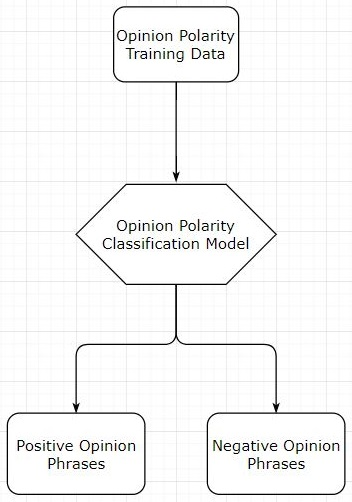
\includegraphics[scale=0.60]{images/opinion_classifier.JPG}
\caption{Classification of positive and negative opinion phrases.}
\end{figure}

For the first approach Britz's (2017) implementation of Kim's "Convolutional Neural Networks (CNN) trained on top of pre-trained word vectors for sentence-level classification tasks" (Kim, 2014)  was considered. This implementation was great and really straight forward to use. A CNN model for text classification was trained on Pang and Lee's publically available labelled movie review data set (Pang \& Lee, 2004). 
For the second approach there are way too many sentiment classifiers publically available online and for this project the library called TextBlob (Loria, 2017) was chosen, since it offers a quite accurate sentiment analyzer with the execution of only a few lines of code. TextBlob has a sentiment classifier model built in the library, thus it classifies opinion phrases as positive or negative (or even neutral).
After both approaches have been tried out, the second approach outperformed the first approach, thus the second approach (TextBlob) made it into the technique's final algorithms system, while the first approach (CNN model) is not used in the current version of the technique.

\subsection{Feature breakdown of all opinion phrases}
Once the polarity of opinion phrases was determined, in order to summarize all positive and negative opinions, one needs to have a feature breakdown of all the opinion phrases classified under the feature that they belong to. This can be accomplished two ways: cross-referencing the list of features identified by the feature extractor, with each opinion phrases' feature word, then creating a list of opinion phrases belonging to each feature extracted or clustering all relation vectors representing the opinion phrases. For the purposes project the easier and more straight forward approach, the cross-referencing approach was implemented into the final algorithm system, with the mindset of keeping things simple. The clustering of opinion phrases is possible and it was done as exploratory data analysis right at the beginning of the research project. A detailed description of such analysis can be found in section 5.1. 

\subsection{Feature Based Opinion Mining System}
Finally, figure 11 shows the summary of all the results. This type of feature breakdown summary is the output of a real feature based opinion mining system.

\begin{figure}
\centering
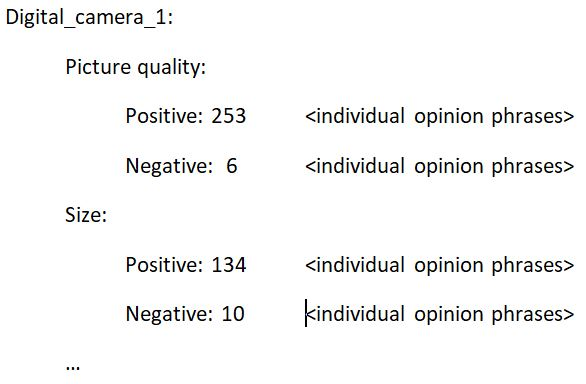
\includegraphics[scale=0.60]{images/fbom_system.JPG}
\caption{Sample output from a Feature based Opinion Mining System.}
\end{figure}

\subsection{The whole system of algorithms and models all together}
To summarize the whole technique in a high level, one paragraph overview, the raw customer reviews get preprocessed in two different ways, then a feature extractor extracts all potential features. After feature extraction, a dependency parser is applied to find a list of dependent words to each feature. All words get converted into high dimensional vectors, with the help of word embedding models. Labelled training data gets pre-processed, then it gets fed into multiple machine learning classification models, which learn the characteristics of opinion phrases in form of relation vectors. After doing so, the feature - dependency word linkage connects each feature with all of its dependency words to form potential relation vectors. The 'Feature - Dependency Word Linkage' creates many non-real feature descriptor relation vectors, which need to be filtered out. With the help of the already trained relation vector classification models most of the non real relation vectors can be filtered out, leaving only the real feature descriptors.  Once all the real feature descriptors have been found, the polarity of opinion phrases is getting classifies as positive or negative. Finally, using a feature breakdown, a summary of all the positive and negative opinions found about each feature of the product present in the customer reviews is created.
In figure 12 one can see how all of the previously mentioned algorithms and techniques work together to form the system of algorithms, that make the whole technique work.

\begin{figure}
\centering
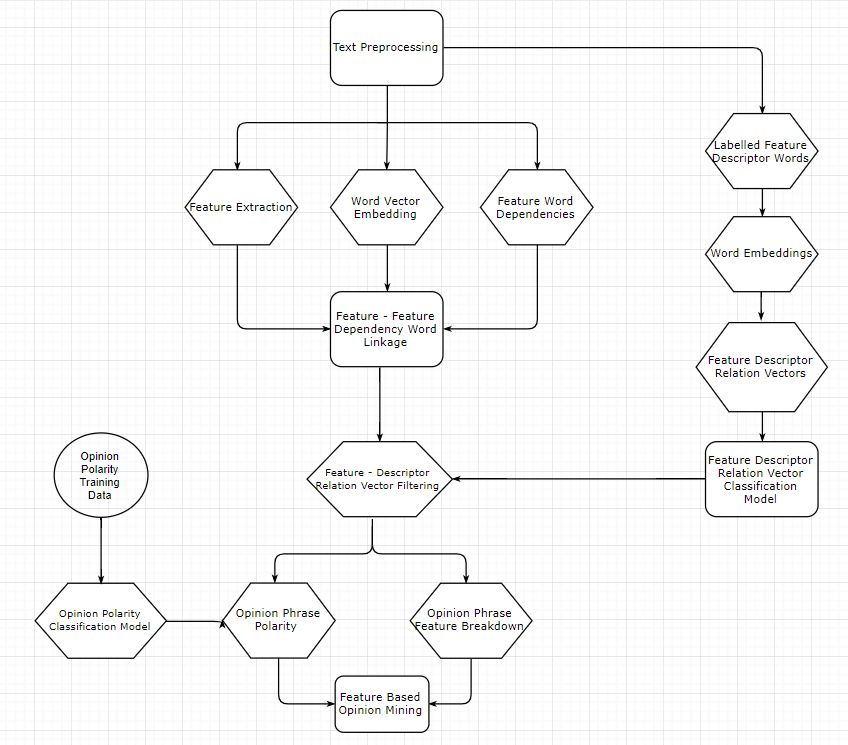
\includegraphics[scale=0.50]{images/full_technique.JPG}
\caption{Diagram of the whole system of algorithms interacting with each other to create a modern Feature based Opinion Mining system.}
\end{figure}



\section{Future Work}
While coming up with features for our tool, we also thought of some ideas, upon which we are yet to perform feasibility analysis and come to a conclusion. These would be great additions to the tool. We are documenting them in this report.
\begin{itemize}
\item Speech-to-text conversion: This feature will allow a user to check his pronunciation by letting him speak into a microphone, and then comparing it with the pronunciation of a native speaker's.
\item Social collaboration: This feature will allow users to discuss about words or phrases on a forum-like platform, thus enabling exchange of more context clues. 
\end{itemize}

%
% The following two commands are all you need in the
% initial runs of your .tex file to
% produce the bibliography for the citations in your paper.

%\bibliographystyle{abbrv}
%\bibliography{sigproc}  % sigproc.bib is the name of the Bibliography in this case


% You must have a proper ".bib" file
%  and remember to run:
% latex bibtex latex latex
% to resolve all references
%
% ACM needs 'a single self-contained file'!
%


\end{document}